\documentclass[%
  class = book,%
  crop = false,%
  float = true,%
  multi = true,%
  preview = false,%
]{standalone}
\usepackage[%
    backend    = biber,%
    style      = chem-acs,%
    autocite   = superscript,%
    backref    = true,%
    biblabel   = brackets,%
    doi        = true,%
    minnames   = 1,%
    maxnames   = 999,%
]{biblatex}
\let\cite\autocite
\DefineBibliographyStrings{english}{%
  backrefpage = {page},% originally "cit. on p."
  backrefpages = {pages},
}
\addbibresource{./paper.bib}
\addbibresource{../5773968.bib}
\addbibresource{../paper_05/psi4numpy.bib}
\usepackage{algorithm}
\usepackage{algpseudocode}
\usepackage{booktabs}
\usepackage{braket}
\onlyifstandalone{\usepackage[margin=1in]{geometry}}
\onlyifstandalone{\raggedbottom}
\usepackage{graphicx}
\usepackage[bookmarks,hyperindex=true,pdfencoding=auto,psdextra]{hyperref}
\usepackage[version=4]{mhchem}
\newcommand{\arlidimer}{\ce{Ar\bond{....}Li+}}
\usepackage[%
    separate-uncertainty = true,%
    multi-part-units = single,%
    range-units = single,%
    retain-explicit-plus = true,%
]{siunitx}
\DeclareSIUnit[number-unit-product = {\,}]\cal{cal}
\DeclareSIUnit\kcal{\kilo\cal}
\usepackage{listings}
\lstset{%
  basicstyle=\ttfamily\footnotesize,%
  breakatwhitespace=true,%
  breaklines=false,%
  frame=none,%
}
\newcommand{\caps}[1]{\uppercase{#1}}
\begin{document}
\chapter[ALMO Linear Response]{A First Principles Approach for Partitioning Linear Response Properties into Additive and Cooperative Contributions}
\label{ch:paper_04}

The text in this chapter has been adapted from \fullcite{Berquist2018}. The author's contribution to the work included deriving the equations, implementing the algorithm, performing all calculations, and writing the manuscript.

\newcommand{\aud}{\si{\bohr\cubed}}
\newcommand{\geomdeftsvp}{\SI{2.4106}{\angstrom}}
\newcommand{\geomdeftsvpd}{\SI{2.4297}{\angstrom}}

\newcommand{\pdalton}{\textsc{Dalton}}
\newcommand{\libresponse}{\texttt{libresponse}}
\newcommand{\psif}{\textsc{Psi4}}
\newcommand{\qchem}{\textsc{Q-Chem}}
\newcommand{\response}{\textsc{Response}}
\newcommand{\op}[1]{\ensuremath{\hat{#1}}}
\newcommand{\mat}[1]{\ensuremath{\mathbf{#1}}}
\newcommand{\Order}[1]{\ensuremath{\mathcal{O}\left(#1\right)}}
\newcommand{\tr}[1]{\ensuremath{{\mathrm{Tr}}\left\{#1\right\}}}
\newcommand{\eq}[1]{eq.~(\ref{#1})}
\newcommand{\citen}[1]{ref.~\parencite{#1}}
\newcommand{\lr}[2]{\braket{\braket{\op{#1}; \op{#2}}}}
\newcommand{\lrs}[4]{\braket{\braket{\op{#1}_{#2}; \op{#3}_{#4}}}}

\section{\texorpdfstring{\caps{Summary}}{Summary}}

We present the analytic implementation of linear response equations on top of absolutely localized molecular orbitals (ALMOs) as part of \libresponse{}, a library for solving the non-orthogonal molecular response equations for arbitrary operators. In the spirit of the original SCF(MI) and TDDFT(MI) formulations, our method is called linear response for molecular interactions, or LR(MI). Charge transfer was discovered to play an equally significant role in both the ground-state and response iterations.

\section{\texorpdfstring{\caps{Introduction}}{Introduction}}
\label{sec:introduction}

Experimental spectroscopy is a powerful tool for understanding the structure and function of molecular systems, especially when combined with theory and computation\cite{AUTSCHBACH200383,NEESE2009526,doi:10.1021/cr2002239}. Absolutely localized molecular orbitals (ALMOs)\cite{Khaliullin2006} and their associated energy decomposition analysis (ALMO-EDA)\cite{Khaliullin2007} provide a intuitive picture of how interactions at the microscopic scale translate to physical insight at the macroscopic scale. ALMO-EDA is capable of separating the total interaction energy of two or more user-defined arbitrary fragments into the following components:

\begin{equation}
  \label{eq:almo-eda}
  \Delta E_{\text{int}} = \Delta E_{\text{gd}} + \Delta E_{\text{frz}} + \Delta E_{\text{pol}} + \Delta E_{\text{CT}},
\end{equation}

where

\begin{itemize}
\item \(\Delta E_{\text{gd}}\) is the energy raising due to the distortion from each fragment's isolated geometry into the cluster geometry;
\item \(\Delta E_{\text{frz}}\) is the ``frozen density'' interaction, which accounts for classical electrostatics and Pauli repulsion between the fragments, and is usually positive;
\item \(\Delta E_{\text{pol}}\) is the polarization energy, which is the self-consistent response of each fragment's electron density in the field of the other fragments, and is always negative;
\item \(\Delta E_{\text{CT}}\) is the charge transfer interaction/energy, and is always negative.
\end{itemize}

This separation is achieved via a constrained self-consistent field calculation, called SCF for molecular interactions (SCF(MI)), producing ALMOs that incorporate fragment polarization but not charge transfer. There are multiple approximations to \(\Delta E_{\text{CT}}\), which can be further broken apart into a perturbative correction and higher-order effects stemming from a self-consistent treatment, where all orbital constraints are lifted and supersystem SCF iterations are performed (equation 5 in \citen{Khaliullin2008}):

\begin{equation}
  \label{eq:almo-eda-ct}
  \Delta E_{\text{CT}} = \Delta E_{\text{CT}}^{\text{RS}} + \Delta E_{\text{CT}}^{\text{HO}}.
\end{equation}

Each of these terms can be broken apart further into a sum of a true electron delocalization term and a BSSE term:

\begin{equation}
  \begin{aligned}
    \label{eq:almo-eda-ct-bsse}
    \Delta E_{\text{CT}}^{\text{RS}} &= \Delta E_{\text{del}}^{\text{RS}} + \Delta E_{\text{BSSE}}^{\text{RS}}, \\
    \Delta E_{\text{CT}}^{\text{HO}} &= \Delta E_{\text{del}}^{\text{HO}} + \Delta E_{\text{BSSE}}^{\text{HO}}.
  \end{aligned}
\end{equation}

Such an energy decomposition is made possible due to the bottom-up construction of ALMOs, where each ALMO is formed from atomic orbitals (AOs) only on a specific fragment, leading to MOs that are spatially localized onto fragments. In a previous work\cite{Brinzer_2015_212425}, we showed that a similar decomposition is possible for peaks in vibrational spectra according to

\begin{equation}
  \begin{aligned}
    \label{eq:almo-frequencies}
    \omega_{\text{tot}} &= \omega_{\text{free}} + \Delta \omega_{\text{int}}, \\
    \Delta \omega_{\text{int}} &= \Delta \omega_{\text{gd}} + \Delta \omega_{\text{frz}} + \Delta \omega_{\text{pol}} + \Delta \omega_{\text{CT}},
  \end{aligned}
\end{equation}

where each term has an analogous meaning to the original ALMO-EDA, except changes in the vibrational frequencies \(\{\omega\}\) rather than the interaction energy are used. We seek a more general decomposition of response properties, starting with those based on linear response (LR), where each \(\omega\) in \eq{eq:almo-frequencies} is replaced with \(\lr{P}{Q}_{\omega_{Q}}\), representing the influence of a perturbation \(\op{Q}\) with frequency \(\omega_{Q}\) on \(\op{P}\).

This is not the first work to seek a fragment- or subsystem-based decomposition of molecular response properties. The LoProp method\cite{doi:10.1063/1.1778131,JCC:JCC20632} starts from canonical orbitals and performs a series of localizations followed by orthogonalizations, leading to atom- and atom pair-centered contributions. While a top-down approach with only post-SCF localization avoids difficulties with a localized SCF implementation, the use of localized charges and dipole moments requires a finite difference approach beyond first derivatives. Several bottom-up approaches, where localized orbitals or subsystems are formed during the SCF iterations, also exist. More closely related to a many-body expansion (MBE) is the fragment molecular orbital (FMO)\cite{MOCHIZUKI2006418} calculation of frequency-dependent polarizabilities. The use of MBE-derived expressions requires a response calculation for each term in the fragment expansion, where ALMO-based LR solves the equations for all fragments simultaneously. Response equations have also been formulated within subsystem density functional theory (sDFT)\cite{Neugebauer_2009_84104,Pavanello_2013_204118}. sDFT requires the use of an additional kinetic energy functional, while ALMO-based LR can be used with all common exchange-correlation functionals. A comprehensive adaptation of response equations up to dynamic first and second hyperpolarizabilities\cite{JCC:JCC540120409} has been performed with nonorthogonal localized molecular orbitals (NOLMOs)\cite{doi:10.1021/acs.jctc.7b00321}. NOLMOs are not connected to an EDA, preventing a property decomposition into EDA-like terms that are the foundation of ALMO-based LR. An attractive fragment-based method designed specifically for the decomposition of molecular interaction energies is symmetry-adapted perturbation theory (SAPT)\cite{doi:10.1021/cr00031a008}, which is systematically improvable due to its foundations in perturbation theory. However, because the fragment orbitals are not variationally optimized together (unlike \(\Delta E_{\text{pol}}^{\text{ALMO-EDA}}\)), the formulation of derivatives even at the uncorrelated monomer approximation (SAPT0) is nontrivial.

The most related methods are those also built on top of ALMOs, specifically ALMO-CIS\cite{Closser_2015_5791}, ALMO-CIS+CT\cite{Ge_2017_44111}, TDDFT(MI)\cite{doi:10.1063/1.4926837}, and LEA-TDDFT\cite{doi:10.1021/acs.jctc.5b00828}. Compared to ALMO-CIS, our method is more consistent with the index restrictions in TDDFT(MI), and similarly to LEA-TDDFT, we can select individual fragments for allowing charge transfer. For this reason, our method is termed linear response for molecular interactions, or LR(MI).

To this end, we have developed \libresponse{}, a molecular response library for non-orthogonal orbitals and arbitrary operators, in the spirit of the \response{} module of \pdalton{}\cite{daltonpaper}. It is capable of both singlet\cite{doi:10.1063/1.454885} and triplet\cite{doi:10.1063/1.457471} response for restricted and unrestricted wavefunctions using Hartree-Fock (HF) or density functional theory (DFT). Properties can be calculated using either the full time-dependent Hartree-Fock (TDHF) or random phase approximation (RPA) equations, or with the configuration interaction with singles (CIS) approximation\cite{doi:10.1021/j100180a030}. Our current implementation is limited to linear response and static properties (\(\omega = 0\)), with both non-linear response and dynamic properties under current development.

\section{\texorpdfstring{\caps{Theory}}{Theory}}
\label{sec:theory}

For the remainder of the paper, unless otherwise stated, the indices \(i,j,k,l,...\) correspond to unoccupied MOs, \(a,b,c,d,...\) correspond to virtual/unoccupied MOs, \(\mu,\nu,\lambda,\sigma,...\) correspond to AOs, and \(I,J,...\) correspond to fragments. There is no distinction between canonical MO and ALMO indices. Comma-separated indices such as \(ia,jb\) correspond to a matrix with a compound index \(ia\) and another compound index \(jb\).

\subsection{Linear response formalism}
\label{ssec:linear-response-formalism}

The linear response of a molecule in its ground state \(\ket{0}\) to perturbations corresponding to operators \(\op{P}\) and \(\op{Q}\) can be written as the sum over all excited states \(\{n\}\),

\begin{equation}
  \lr{P}{Q}_{\omega}
  =
  - \sum_{n > 0} \;
    \left[
      \frac{\braket{0|\op{P}|n} \braket{n|\op{Q}|0}}{\omega_{n} - \omega}
    + \frac{\braket{0|\op{Q}|n} \braket{n|\op{P}|0}}{\omega_{n} + \omega}
    \right],
\end{equation}

where \(\omega\) is the frequency of the perturbation \(\op{Q}\) and \(\omega_{n} = E_{n} - E_{0}\). Examples of second-order response properties include the polarizability (\(\op{P} = \op{Q} = \op{\mu}\)), magnetizability (\(\op{P} = \op{Q} = \op{m}\)), vibrational frequencies (\(\op{P} = \op{Q} = \op{x}\)), etc. This paper focuses on molecular response within the static limit (\(\omega = 0\)),

\begin{equation}
  \lr{P}{Q}_{0}
  =
  - \tr{\mat{P}^{\dagger} \mat{G}^{-1} \mat{Q}}
  =
  - \tr{\mat{P}^{\dagger} \mat{X}},
\end{equation}

where \((\mat{P})_{ia} = \braket{i|\op{P}|a}\) and \((\mat{Q})_{ia} = \braket{i|\op{Q}|a}\). \(\mat{X} = \mat{G}^{-1} \mat{Q}\) is the ``response vector'' corresponding to orbital rotations induced by perturbation \(\op{Q}\). The orbital Hessian matrix \(\mat{G}\) is defined as

\begin{equation}
  \begin{aligned}
    ^{RR}\mat{G}^{\sigma} &= \mat{A}^{\sigma} + \mat{B}^{\sigma} \\
    ^{II}\mat{G}^{\sigma} &= \mat{A}^{\sigma} - \mat{B}^{\sigma}
  \end{aligned}
\end{equation}
for real (\(R\)) and imaginary (\(I\)) perturbations, respectively\cite{doi:10.1080/00268976.2015.1024182}. The spin case \(\sigma\) can either be singlet (\(\sigma = s\)) or triplet (\(\sigma = t\)) depending on whether the perturbation operator conserves or flips spin, respectively:

\begin{equation}
  \begin{aligned}
    A^{s}_{ia,jb} &= \Delta_{ia} + 2(ia|jb) - (ij|ab) \\
    A^{t}_{ia,jb} &= \Delta_{ia} - (ij|ab)
  \end{aligned}
\end{equation}

\begin{equation}
  \begin{aligned}
    B^{s}_{ia,jb} &= 2(ia|jb) - (ib|ja) \\
    B^{t}_{ia,jb} &= - (ib|ja)
  \end{aligned}
\end{equation}

where \(\Delta_{ia} = (\varepsilon_{a} - \varepsilon_{i}) \delta_{ia,jb}\) is an orbital energy difference. The CIS or Tamm-Dancoff approximation (TDA) is recovered when \(\mat{B} = \mat{0}\). Rather than directly inverting the orbital Hessian, which would cost \Order{o^3 v^3}, one solves iteratively for \(\mat{X}\) by expanding the inverse, for example in the real singlet case

\begin{equation}
  \label{eq:update}
  X_{ia}^{(n+1)}
  =
  \frac{Q_{ia} - \left[4(ia|jb) - (ij|ab) - (ib|ja)\right] X_{jb}^{(n)}}
       {\Delta_{ia}}
\end{equation}

Repeated indices imply summation (Einstein sum convention). Here, the superscript in parentheses denotes the iteration number. To avoid the expensive transformation of two-electron repulsion integrals from atomic orbital into molecular orbital basis, one performs the contraction over orbital pair \(jb\) in the atomic orbital basis,

\begin{equation}
  \left(\mat{A}^{s} + \mat{B}^{s}\right)_{ia,jb} X_{jb}
  =
  C_{\mu i}
  \left[
    4 (\mu\nu|\lambda\sigma) D_{\lambda\sigma}^{X}
    - (\mu\lambda|\nu\sigma) D_{\lambda\sigma}^{X}
    - (\mu\sigma|\lambda\nu) D_{\lambda\sigma}^{X}
  \right]
  C_{\nu a}
\end{equation}

with the perturbed density matrix \(D_{\mu\nu}^{X} = C_{\lambda j} X_{jb} C_{\sigma b}\).

To work with \emph{non-orthogonal orbitals}, we replace the \(\Delta_{ia}^{-1}\) denominator in \eq{eq:update} with a full matrix inversion of

\begin{equation}
  \label{eq:energy-denominator}
  E_{ia,jb} = F_{ab}S_{ij} - F_{ij}S_{ab},
\end{equation}

where \(\mat{F}\) and \(\mat{S}\) are the MO-basis Fock and overlap matrix, respectively

\subsection{Adaptation of linear response equations for absolutely localized MOs}
\label{ssec:almo-adaptation}

The first requirement for adapting the non-orthogonal linear response equations to the ALMO formalism is the projection of the occupied subspace from the virtual subspace. This is because the original fragment-local virtual ALMOs are not orthogonal to occupied ALMOs on other fragments. We form ``modified'' or ``projected'' virtual orbitals,

\begin{equation}
  \label{eq:projected-virtuals}
  \ket{\phi_{a}} = N_{a} \left( 1 - \op{D}_{\text{occ}} \right) \ket{\psi_{a}}
\end{equation}

where \(\op{D}_{\text{occ}} \rightarrow (\mat{D}_{\text{occ}})_{\mu\nu} = C_{\mu i} C_{\nu i}\). Otherwise, this contamination would manifest as spurious low-lying excited states, leading to artificial poles in the polarizability. This requirement for projection is unimportant for ground-state SCF(MI) calculations, where the virtual orbitals do not have an effect on the final result (energy).

The second requirement is to maintain consistency with the fragment-local nature of SCF(MI), where CT is not allowed. Each occupied-virtual MO contribution to the molecular response is restricted to be within the same fragment. This corresponds to forcing all \(ia\) (or \(jb\)) pairs to be zero when \(i \in F_{I}, a \in (F_{J} \neq F_{I})\). Algorithmically, we do this by always working in the full CT-allowed basis, then zeroing out CT-disallowed matrix elements. For the energy denominator, the zero rows and columns must be removed to avoid introducing artificial singularities. The advantage of working in the full CT basis and zeroing matrix elements is twofold: it prevents code duplication due to no need for separate non-orthogonal and ALMO-based response routines, and it enables selection of individual fragments to quantify their CT contribution to the final response property. This is in contrast to ALMO-CIS+CT\cite{Ge_2017_44111}, which starts from the reduced CT-disallowed basis and adds a distance-dependent CT correction. An outline of the algorithm is available in the SI.

Perhaps the most important fundamental distinction between our formulation of the ALMO response equations and the ALMO-CIS formulation is in the two-electron contribution, where we restrict MO indices but do not restrict AO indices. This means that for a given \(J_{\mu\nu}^{X} = (\mu\nu|\lambda\sigma)D_{\lambda\sigma}^{X}\), summations run over AO indices on all fragments, and both \((\mu\nu|\lambda\sigma)\) and \(D_{\lambda\sigma}^{X}\) for \(\lambda\in F_{I}, \sigma\in (F_{J} \neq F_{I})\) may be non-zero. Additionally, AO indices cannot be restricted due to the projection in \eq{eq:projected-virtuals}, where each MO can have contributions from all AOs.

In principle, the ALMO formulation presented here can be extended to arbitrary-order response, as long as each compound \(ia\) index is constrained to be within a fragment.

\subsection{Decomposition of linear response properties into local contributions and interaction mechanisms}
\label{ssec:decomp-line-resp}

As with other localized orbital schemes, there is a question of how to define charge transfer. Our implementation allows for the introduction of CT in several stages. This allows for further decomposition of the CT term into qualitative contributions from individual fragments. This is done by starting from the polarized SCF(MI) wavefunction and allowing transitions between the occupied space of a single fragment into the virtual space of all fragments. This can be denoted as ``frz + pol + CT(\(F \rightarrow\) all)'', where \(F\) is an individual fragment. The difference between this result and ``frz + pol'' can be viewed as how important CT is for that specific fragment \(F\). From the symmetry-adapted perturbation theory\cite{STONE2009201} perspective, it can also be viewed as a BSSE correction; the larger the difference, the more deficient the fragment-localized basis is. CT can also be allowed during the response calculation even if it was not during the wavefunction calculation; this corresponds to performing non-orthogonal response with no restrictions using the polarized SCF(MI) wavefunction, represented as ``frz + pol + CT(all \(\rightarrow\) all) [blocked]''. The sum over all fragments should be qualitatively equal to ``frz + pol + CT(all \(\rightarrow\) all) [blocked]'', though it will not be exactly equal due to higher-order effects, similar to the \(\Delta E_{\text{CT}}^{\text{HO}}\) term in ALMO-EDA. Finally, ``frz + pol + CT(all \(\rightarrow\) all) [blocked]'' corresponds to an unrestricted response calculation on top of the fully-relaxed SCF wavefunction, analogous to a supersystem calculation. The difference between the blocked result and the supersystem result shows the effect of allowing CT in the underlying wavefunction.

This multi-step decomposition of the CT term is similar to our previous work on the effect of CT on the vibrational spectra of \ce{CO2} in ionic liquids\cite{Brinzer_2015_212425,Berquist_2017_208}. Being able to turn CT on and off during the geometry optimization and numerical Hessian calculation allowed us to see how CT contributes to the potential energy surface at multiple stages, but our analytic formulation of the response equations has significant advantages. It enables the identification of fragment-specific contributions to the total response, which is not possible in a numerical response calculation, even with an underlying SCF(MI) wavefunction. This is in addition to all the other advantages of solving analytic rather than numerical equations, namely calculation time, uncoupled and perturbative approximations to fully iterative results, lack of finite-difference error, frequency-dependent perturbations, and response to applied magnetic fields without complex energies; see \citen{gauss2000} for a discussion.

Borrowing terminology from \citen{Berquist_2017_208}, CT may enter the response calculation through multiple mechanisms. We consider two: the ``wave\-function mechanism'', where CT is (dis)\-allowed during the SCF iterations, corresponding to either an SCF(MI) or a canonical SCF calculation, and the ``response mechanism'', where CT is (dis)\-allowed during the response calculation by restricting occupied-virtual MO contributions to be within fragments as discussed in section~\ref{ssec:almo-adaptation}. This results in four principal permutations of (dis)\-allowing CT effects, abbreviated as ``\(a/b\)'', where \(a\) represents the wavefunction mechanism, \(b\) represents the response mechanism, and \(a,b\in\{\text{on},\text{off}\}\):

\begin{itemize}
\item ``on/on'' is a standard response calculation, and is the ``frz + pol + CT(all \(\rightarrow\) all) [super]'' result.
\item ``off/off'' is the most consistent with SCF(MI) and TDDFT(MI), and is the ``frz + pol'' result.
\item ``off/on'' attempts to recover CT effects during the response calculation that are missing from the underlying SCF(MI) wavefunction, and is the ``frz + pol + CT(all \(\rightarrow\) all) [blocked]'' result. This is not the same as the single perturbative Roothaan step (RS) correction in SCF(MI), but is a fully-iterative response calculation on top of ALMOs.
\item ``on/off'' corresponds to allowing CT during SCF iterations but not the response calculations. This decomposition is not considered, as neither the occupied nor the virtual canonical orbitals can generally be assigned to specific fragments.
\end{itemize}

For the purposes of this work, we also do not consider the effect of disallowing CT during geometry optimization through the ``geometry mechanism'', though in principle it is technically feasible and potentially non-negligible. See \citen{Mao_2017_5944} for an in-depth analysis of the different potential energy surfaces that comprise ALMO-EDA. Neglecting the geometry mechanism means our approach is consistent with a vertical decomposition rather than an adiabatic one.

\section{\texorpdfstring{\caps{Methods}}{Methods}}
\label{sec:methods}

HF was used for all calculations as a proof of concept to avoid spurious overdelocalization and CT effects due to self-interaction error. As a result, it should provide a lower bound on any possible CT effects during the SCF(MI) calculation. For basis sets, we chose the Karlsruhe def2- family\cite{Weigend_2005_3297,Rappoport_2010_134105}, in particular def2-SVP and def2-SVPD. It is well-known that the original ALMO procedure has a strong basis-set dependence, with overestimation of \(\Delta E_{\text{pol}}\) and underestimation of \(\Delta E_{\text{CT}}\) due to the overlapping tails of AOs on different fragments, allowing electron density to ``leak'' across fragments during SCF(MI)\cite{doi:10.1063/1.4792434}. As a result, there is no clear basis set limit to \(\Delta E_{\text{pol}}\). This informs our basis set choices, which should give qualitatively correct results within the original ALMO definition, with a check on minimal augmentation optimized for use in electric field response calculations.

For a test property, we chose the static dipole polarizability, defined as

\begin{equation}
  \alpha_{ab}(0) = -\lrs{\mu}{a}{\mu}{b}_{0} = -\left.\frac{\partial^{2} E}{\partial \varepsilon_a \partial \varepsilon_b}\right|_{\varepsilon_{a},\varepsilon_{b}=0},
\end{equation}

where \(a,b \in \{x,y,z\}\) and the energy derivative method based on derivatives with respect to applied electric fields \(\varepsilon\) is equivalent to the linear response calculation.

For a test system, the argon\textemdash{}lithium cation dimer, \arlidimer{}, was chosen due to the reasonable polarizability of the bare (closed-shell) argon atom, which should be quantitatively influenced by the almost unscreened nuclear charge of the lithium cation. The optimized distances are \geomdeftsvp{} using def2-SVP and \geomdeftsvpd{} using def2-SVPD. For the distance dependence results, points are spaced at \SI{0.05}{\angstrom} from \SIrange{1.25}{5.00}{\angstrom}, then spaced at \SI{0.25}{\angstrom} from \SIrange{5.00}{10.00}{\angstrom}.

All calculations were performed using a development version of \qchem{}\cite{Shao2015} compiled with \libresponse{}, our generalized non-orthogonal molecular response library. Thresholds were set to \num{e-14} for integral screening, \num{e-11} for the DIIS error norm in SCF convergence, and \num{e-8} for the DIIS error norm in the analytic response iterations. The Stoll projector equations were used for minimizing the underlying SCF(MI) wavefunction\cite{Stoll_1980_169,Khaliullin2006}. For numerical polarizability calculations, 2nd-order finite difference from energies was used, unless otherwise stated, as differences between 1st- and 2nd-order results were below \num{e-7} \aud{} in all cases. Both 1st- and 2nd-order finite difference polarizability calculations used a finite field step size of \num{1.88973e-5} \aud{}. All SCF(MI) analytic polarizability calculations use projected virtual orbitals as defined by \eq{eq:projected-virtuals}.

\section{\texorpdfstring{\caps{Results and Discussion}}{Results and Discussion}}
\label{sec:results-and-discussion}

\subsection{Equilibrium distance}
\label{ssec:results-equilibrium-distance}

\begin{table}
  \centering
  \caption[Argon\textemdash{}lithium cation dimer polarizabilities using HF/def2-SVP]{Polarizability results for the argon\textemdash{}lithium cation dimer at the HF/def2-SVP level. The geometry is optimized at the same level. All values have units of \aud{}.}
  \label{table:polarizability-results-def2-svp}
  \IfStandalone{\begin{tabular}{lrrrrrr}%
\toprule%
&\multicolumn{3}{c}{analytical}&\multicolumn{3}{c}{numerical}\\%
\cmidrule{2-4}\cmidrule{5-7}%
def2-SVP&\(\alpha_{\perp}\)&\(\alpha_{\parallel}\)&\(\alpha_{\text{iso}}\)&\(\alpha_{\perp}\)&\(\alpha_{\parallel}\)&\(\alpha_{\text{iso}}\)\\%
\midrule%
monomer A (\ce{Ar})&4.3702&4.3702&4.3702&4.3702&4.3702&4.3702\\%
monomer B (\ce{Li+})&0.1593&0.1593&0.1593&0.1593&0.1593&0.1593\\%
A + B&4.5295&4.5295&4.5295&4.5295&4.5295&4.5295\\%
frz + pol&4.5042&4.5581&4.5222&4.5036&4.5696&4.5256\\%
+ CT(A \(\rightarrow\) all)&4.7040&5.5191&4.9757&\textemdash{}&\textemdash{}&\textemdash{}\\%
+ CT(B \(\rightarrow\) all)&0.1594&0.1586&0.1591&\textemdash{}&\textemdash{}&\textemdash{}\\%
+ CT(all \(\rightarrow\) all) [blocked]&4.8409&5.7540&5.1452&\textemdash{}&\textemdash{}&\textemdash{}\\%
+ CT(all \(\rightarrow\) all) [super]&5.2142&7.8649&6.0978&5.2142&7.8649&6.0978\\%
\bottomrule%
\end{tabular}
}{\begin{tabular}{lrrrrrr}%
\toprule%
&\multicolumn{3}{c}{analytical}&\multicolumn{3}{c}{numerical}\\%
\cmidrule{2-4}\cmidrule{5-7}%
def2-SVP&\(\alpha_{\perp}\)&\(\alpha_{\parallel}\)&\(\alpha_{\text{iso}}\)&\(\alpha_{\perp}\)&\(\alpha_{\parallel}\)&\(\alpha_{\text{iso}}\)\\%
\midrule%
monomer A (\ce{Ar})&4.3702&4.3702&4.3702&4.3702&4.3702&4.3702\\%
monomer B (\ce{Li+})&0.1593&0.1593&0.1593&0.1593&0.1593&0.1593\\%
A + B&4.5295&4.5295&4.5295&4.5295&4.5295&4.5295\\%
frz + pol&4.5042&4.5581&4.5222&4.5036&4.5696&4.5256\\%
+ CT(A \(\rightarrow\) all)&4.7040&5.5191&4.9757&\textemdash{}&\textemdash{}&\textemdash{}\\%
+ CT(B \(\rightarrow\) all)&0.1594&0.1586&0.1591&\textemdash{}&\textemdash{}&\textemdash{}\\%
+ CT(all \(\rightarrow\) all) [blocked]&4.8409&5.7540&5.1452&\textemdash{}&\textemdash{}&\textemdash{}\\%
+ CT(all \(\rightarrow\) all) [super]&5.2142&7.8649&6.0978&5.2142&7.8649&6.0978\\%
\bottomrule%
\end{tabular}
}
\end{table}

\begin{table}
  \centering
  \caption[Argon\textemdash{}lithium cation dimer polarizabilities using HF/def2-SVPD]{Polarizability results for the argon\textemdash{}lithium cation dimer at the HF/def2-SVPD level. The geometry is optimized at the same level. All values have units of \aud{}.}
  \label{table:polarizability-results-def2-svpd}
  \IfStandalone{\begin{tabular}{l|rrr|rrr}%
\hline%
\hline%
\ce{Ar\bond{....}Li+}&\multicolumn{3}{c}{analytical}&\multicolumn{3}{c}{numerical}\\%
\hline%
def2-SVPD&\(\alpha_{\perp}\)&\(\alpha_{\parallel}\)&\(\alpha_{\text{iso}}\)&\(\alpha_{\perp}\)&\(\alpha_{\parallel}\)&\(\alpha_{\text{iso}}\)\\%
\hline%
monomer A (\ce{Ar})&10.3735&10.3735&10.3735&10.3735&10.3735&10.3735\\%
monomer B (\ce{Li+})&0.1603&0.1603&0.1603&0.1603&0.1603&0.1603\\%
A + B&10.5338&10.5338&10.5338&10.5338&10.5338&10.5338\\%
frz + pol&10.0787&10.6399&10.2658&10.0875&10.6599&10.2783\\%
frz + pol + CT(A \(\rightarrow\) all)&10.0157&10.4900&10.1738&{-}{-}&{-}{-}&{-}{-}\\%
frz + pol + CT(B \(\rightarrow\) all)&0.1606&0.1614&0.1609&{-}{-}&{-}{-}&{-}{-}\\%
frz + pol + CT(all \(\rightarrow\) all) [blocked]&10.1395&10.8004&10.3598&{-}{-}&{-}{-}&{-}{-}\\%
frz + pol + CT(all \(\rightarrow\) all) [super]&10.0724&11.0645&10.4031&10.0724&11.0645&10.4031\\%
\hline%
\hline%
\end{tabular}}{\begin{tabular}{l|rrr|rrr}%
\hline%
\hline%
\ce{Ar\bond{....}Li+}&\multicolumn{3}{c}{analytical}&\multicolumn{3}{c}{numerical}\\%
\hline%
def2-SVPD&\(\alpha_{\perp}\)&\(\alpha_{\parallel}\)&\(\alpha_{\text{iso}}\)&\(\alpha_{\perp}\)&\(\alpha_{\parallel}\)&\(\alpha_{\text{iso}}\)\\%
\hline%
monomer A (\ce{Ar})&10.3735&10.3735&10.3735&10.3735&10.3735&10.3735\\%
monomer B (\ce{Li+})&0.1603&0.1603&0.1603&0.1603&0.1603&0.1603\\%
A + B&10.5338&10.5338&10.5338&10.5338&10.5338&10.5338\\%
frz + pol&10.0787&10.6399&10.2658&10.0875&10.6599&10.2783\\%
frz + pol + CT(A \(\rightarrow\) all)&10.0157&10.4900&10.1738&{-}{-}&{-}{-}&{-}{-}\\%
frz + pol + CT(B \(\rightarrow\) all)&0.1606&0.1614&0.1609&{-}{-}&{-}{-}&{-}{-}\\%
frz + pol + CT(all \(\rightarrow\) all) [blocked]&10.1395&10.8004&10.3598&{-}{-}&{-}{-}&{-}{-}\\%
frz + pol + CT(all \(\rightarrow\) all) [super]&10.0724&11.0645&10.4031&10.0724&11.0645&10.4031\\%
\hline%
\hline%
\end{tabular}}
\end{table}

Tables~\ref{table:polarizability-results-def2-svp}~and~\ref{table:polarizability-results-def2-svpd} show equilibrium distance results for the argon\textemdash{}lithium cation dimer at the HF/def2-SVP and HF/def2-SVPD levels, respectively. Due to molecular symmetry, two of the three polarizability tensor principal components are identical; these correspond to the perpendicular polarizability \(\alpha_{\perp}\), or how easy it is to shift the electron density perpendicular to the interatomic axis. The parallel polarizability \(\alpha_{\parallel}\) corresponds to the principal component that lies along the axis of interaction between the two atoms and corresponds to the bond polarizability. Monomer A and B refer to the isolated atoms; parallel and perpendicular axes have no meaning here due to their spherical symmetry, as all principal components are identical. An approximation to the frozen density interaction in response is the sum of the response of the isolated fragments (atoms), shown as ``A + B''. Note that this is not the true frozen monomer response\cite{Mao_2017_5944}. ``frz + pol'' is where CT is disallowed between fragments using the algorithm described above, consistent with the original SCF(MI) and conceptually analogous to TDDFT(MI). The remaining entries are those described in section~\ref{ssec:decomp-line-resp}.

\subsubsection{Validation of analytic ALMO results}
\label{sssec:results-validation}

As a correctness check, our analytic formulation is validated against finite-field calculations in the last three columns. An advantage of the analytic formulation is the ability to further decompose the CT term; it is not possible to perform the ``CT(A \(\rightarrow\) all)'', ``CT(B \(\rightarrow\) all)'', and ``CT(all \(\rightarrow\) all) [blocked]'' calculations with a finite-field approach. For both basis sets presented, there is no quantitative difference between the analytic and numerical polarizabilities except for ``frz + pol''. This should not be interpreted as an error, since our definition of the response equations differs from the no-CT formulation presented by ALMO-CIS, and there is a slight delocalization of the virtual space due to the projection (see section~\ref{sec:conclusions-and-future-work}). Still, the largest percent difference is 0.25\% and 0.19\% in \(\alpha_{\parallel}\) for def2-SVP and def2-SVPD, respectively, showing our definition should be valid as long as the ALMO approximation holds.

\subsubsection{CT mechanism analysis}
\label{sssec:ct-mechanism-analysis}

From tables~\ref{table:polarizability-results-def2-svp}~and~\ref{table:polarizability-results-def2-svpd}, the importance of charge transfer via both the wavefunction and response mechanisms can be calculated as the difference between ``frz + pol'', ``CT(all \(\rightarrow\) all) [blocked]'', and ``CT(all \(\rightarrow\) all) [super]''; these are ``off/off'', ``off/on'', and ``on/on'', respectively. The effect of each mechanism is shown in table~\ref{tab:mechanism-percentage-changes}.

\begin{table}
  \centering
  \caption[Percentage changes in argon\textemdash{}lithium cation dimer \(\alpha_{\parallel}\) due to the two CT mechanisms]{Percentage changes in \(\alpha_{\parallel}\) due to the two CT mechanisms. The reference (denominator) polarizability used is shown in \textit{italics}. All calculations used a bond length of \geomdeftsvpd{}.}
  \label{tab:mechanism-percentage-changes}
  \begin{tabular}{ccc}
    \toprule
                                           & \multicolumn{2}{c}{basis set} \\
    percentage change due to mechanism     & def2-SVP    & def2-SVPD       \\
    \midrule
    response (\textit{off/on} - off/off)   & 20.8        & 1.5             \\
    wavefunction (\textit{on/on} - off/on) & 26.8        & 2.4             \\
    \bottomrule
  \end{tabular}
\end{table}

For def2-SVP, it is clear that each successive relaxation of CT restrictions has a non-negligible effect on the final property, where \(\alpha_{\parallel}^{\text{frz + pol}}\) is 58.0\% and 96.2\% of the supermolecular value for the two basis sets. This representation makes it clear that in addition to larger polarizabilities (\(\sim 2 \times\)), there are other fundamental differences caused by the use of diffuse functions in def2-SVPD.

% Viewed another way, if CT does not contribute strongly to the interaction of fragments, a large fraction of the supermolecular or canonical SCF result should recovered regardless of the CT restriction level, in the spirit of the original SCF(MI) approximation\cite{Khaliullin2006}. These fractions are shown in table~\ref{tab:mechanism-percentage-of-super}

% \begin{table}
%   \begin{tabular}{ccc}
%     \toprule
%                                 & \multicolumn{2}{c}{basis set} \\
%     \fxnote{?}   & def2-SVP    & def2-SVPD   \\
%     \midrule
%     (off/off) / (off/on)        & 79.2        & 98.5            \\
%     (off/off) / (on/on)         & 58.0        & 96.2            \\
%     (off/on) / (on/on)          & 73.2        & 97.6            \\
%     \bottomrule
%   \end{tabular}
%   \caption{Percent contribution of each mechanism \fxnote{?}. All calculations used a bond length of \geomdeftsvpd{}.}
%   \label{tab:mechanism-percentage-of-super}
% \end{table}

Calculated this way, the wavefunction mechanism may include some higher-order effects, as the pure wavefunction mechanism, calculated as ``on/off'' - ``off/off'',  cannot be isolated due to the ``on/off'' term (see section~\ref{ssec:decomp-line-resp}). The size of these higher-order effects in the wavefunction can be estimated by the percent contribution of higher-order effects in ALMO-EDA charge transfer, shown in table~\ref{tab:almo-eda-higher-order-pct-of-ct}.

\begin{table}
  \centering
  \caption[Higher-order ALMO-EDA charge transfer in argon\textemdash{}lithium cation dimer]{Percentage of ALMO-EDA charge transfer due to higher-order effects, calculated as \(100 * \frac{\Delta E_{\text{CT}}^{\text{HO}}}{\Delta E_{\text{CT}}^{\text{RS}} + \Delta E_{\text{CT}}^{\text{HO}}}\). All calculations used a bond length of \geomdeftsvpd{}.}
  \label{tab:almo-eda-higher-order-pct-of-ct}
  \begin{tabular}{ccc}
    \toprule
                    & \multicolumn{2}{c}{basis set} \\
    BSSE corrected? & def2-SVP    & def2-SVPD   \\
    \midrule
    no              & 24.2        & 17.1        \\
    yes             & 25.0        & 19.4        \\
    \bottomrule
  \end{tabular}
\end{table}

Using the uncorrected results for consistency, the new estimates of percentage changes due to the wavefunction mechanism become 20.3\% and 2.0\%, showing the presence of CT in the underlying wavefunction and in the response calculation are equally important in predicting molecular properties.

\subsubsection{Basis set dependence}
\label{sssec:basis-set-dependence}

The results in table~\ref{tab:mechanism-percentage-changes} show that charge transfer, or electron delocalization across fragments, is relatively unimportant when using the diffuse basis set. This may be indicative of either basis set incompleteness or overlap between the tails of the diffuse basis functions (see section~\ref{sec:methods}). The former argument is supported by the BSSE term being 50\% of the total CT term with def2-SVP but only 18\% with def2-SVPD, while the latter argument is supported by a doubling of \(\Delta E_{\text{pol}}\) from \SIrange{-3.3}{-6.6}{\kcal\per\mol} when adding the diffuse functions (see the SI for all ALMO-EDA results).

To investigate these effects directly on the polarizability, rather than through an EDA, table~\ref{tab:basis-set-dependence} shows the decoupled effect of the nuclear charge and basis functions provided by the lithium cation on the argon. Since the lithium cation is not very polarizable (\(\alpha^{\ce{Li+}}\) is \(\approx 4\%\) of \(\alpha^{\ce{Ar}}\) at the HF/def2-SVP level), only effects on the argon atom are considered. Also presented are the lowest singlet and triplet excitation energies calculated using RPA (TD-HF). Percentages of each value compared to the full \arlidimer{} result within each basis set are shown in the SI.

In order to test the importance of nuclear charge without the influence of basis functions, the ``PC(+)'' and ``PC(-)'' entries represent replacing the lithium atom with positive and negative point charges of unit magnitude, respectively. To test the importance of the basis set without the influence of a nuclear charge, ``Gh(Li)'' represents replacing the full lithium atom with only its basis functions, leaving a ``ghost atom'' with no (effective) nuclear charge. This should separate the \arlidimer{} interaction into a purely electrostatic effect from the nucleus, a delocalization-like effect due to increased spatial flexibility for motion of electrons during SCF and response iterations, and some non-additive effects.

\begin{table}
  \centering
  \caption[Point charge and basis function contributions to argon\textemdash{}lithium cation dimer polarizabilities]{Decomposition of polarizabilities into point charge and basis function contributions. All calculations used canonical MOs and a distance of \geomdeftsvpd{} from argon to the other center(s).}
  \label{tab:basis-set-dependence}
  \IfStandalone{\begin{tabular}{llrrrrr}
\toprule
 basis set &                          structure & \(\alpha_{\perp}\) (a.u.) & \(\alpha_{\parallel}\) (a.u.) & \(\bar{\alpha}\) (a.u.) & \(^{\text{t}}E_{0 \rightarrow \text{lowest}}^{\text{RPA}}\) (eV) & \(^{\text{s}}E_{0 \rightarrow \text{lowest}}^{\text{RPA}}\) (eV) \\
\midrule
  def2-SVP &   \ce{Ar\bond{....}PC(\mathrm{-})} &                      4.38 &                          4.35 &                    4.37 &                                                            23.26 &                                                            25.09 \\
  def2-SVP &                            \ce{Ar} &                      4.37 &                          4.37 &                    4.37 &                                                            23.69 &                                                            25.50 \\
  def2-SVP &   \ce{Ar\bond{....}PC(\mathrm{+})} &                      4.36 &                          4.38 &                    4.37 &                                                            23.42 &                                                            25.24 \\
  def2-SVP &  \ce{Ar\bond{....}\mathrm{Gh}(Li)} &                      4.89 &                          6.23 &                    5.34 &                                                            12.26 &                                                            12.58 \\
  def2-SVP &              \ce{Ar\bond{....}Li+} &                      5.21 &                          7.88 &                    6.10 &                                                            11.90 &                                                            12.18 \\
 def2-SVPD &   \ce{Ar\bond{....}PC(\mathrm{-})} &                     10.94 &                         10.33 &                   10.74 &                                                            10.92 &                                                            11.68 \\
 def2-SVPD &                            \ce{Ar} &                     10.37 &                         10.37 &                   10.37 &                                                            12.61 &                                                            13.22 \\
 def2-SVPD &   \ce{Ar\bond{....}PC(\mathrm{+})} &                     10.04 &                         11.94 &                   10.67 &                                                             9.90 &                                                            10.48 \\
 def2-SVPD &  \ce{Ar\bond{....}\mathrm{Gh}(Li)} &                     10.39 &                         10.42 &                   10.40 &                                                            12.05 &                                                            12.41 \\
 def2-SVPD &              \ce{Ar\bond{....}Li+} &                     10.07 &                         11.06 &                   10.40 &                                                            11.98 &                                                            12.34 \\
\bottomrule
\end{tabular}
}{\begin{tabular}{llrrrrr}
\toprule
 basis set &                          structure & \(\alpha_{\perp}\) (a.u.) & \(\alpha_{\parallel}\) (a.u.) & \(\bar{\alpha}\) (a.u.) & \(^{\text{t}}E_{0 \rightarrow \text{lowest}}^{\text{RPA}}\) (eV) & \(^{\text{s}}E_{0 \rightarrow \text{lowest}}^{\text{RPA}}\) (eV) \\
\midrule
  def2-SVP &   \ce{Ar\bond{....}PC(\mathrm{-})} &                      4.38 &                          4.35 &                    4.37 &                                                            23.26 &                                                            25.09 \\
  def2-SVP &                            \ce{Ar} &                      4.37 &                          4.37 &                    4.37 &                                                            23.69 &                                                            25.50 \\
  def2-SVP &   \ce{Ar\bond{....}PC(\mathrm{+})} &                      4.36 &                          4.38 &                    4.37 &                                                            23.42 &                                                            25.24 \\
  def2-SVP &  \ce{Ar\bond{....}\mathrm{Gh}(Li)} &                      4.89 &                          6.23 &                    5.34 &                                                            12.26 &                                                            12.58 \\
  def2-SVP &              \ce{Ar\bond{....}Li+} &                      5.21 &                          7.88 &                    6.10 &                                                            11.90 &                                                            12.18 \\
 def2-SVPD &   \ce{Ar\bond{....}PC(\mathrm{-})} &                     10.94 &                         10.33 &                   10.74 &                                                            10.92 &                                                            11.68 \\
 def2-SVPD &                            \ce{Ar} &                     10.37 &                         10.37 &                   10.37 &                                                            12.61 &                                                            13.22 \\
 def2-SVPD &   \ce{Ar\bond{....}PC(\mathrm{+})} &                     10.04 &                         11.94 &                   10.67 &                                                             9.90 &                                                            10.48 \\
 def2-SVPD &  \ce{Ar\bond{....}\mathrm{Gh}(Li)} &                     10.39 &                         10.42 &                   10.40 &                                                            12.05 &                                                            12.41 \\
 def2-SVPD &              \ce{Ar\bond{....}Li+} &                     10.07 &                         11.06 &                   10.40 &                                                            11.98 &                                                            12.34 \\
\bottomrule
\end{tabular}
}
\end{table}

As expected, compared to a bare argon atom, the presence of a ghost function both increases the polarizability and decreases the first excitation energy. Intuitively, there are now additional molecular orbitals within reasonable spatial distance that electron density can spread on to as part of the ground-state calculation and can be excited to as part of the excited-state calculation. The difference is much less pronounced for the diffuse basis, where it is the presence of point charges that has the larger effect. This indicates that there is overlap with the tails of only the additional diffuse basis functions at the distance of the lithium center, and is caused by basis set incompleteness present even at the canonical SCF level. The point charges are in comparatively empty space in the non-diffuse basis, and the ghost function is unimportant for the diffuse basis. There, \(\alpha_{\parallel}^{\text{PC(+)}} \gg \alpha_{\parallel}^{\arlidimer{}}\) due to electron screening on the lithium atom, which leads to a reduced effective nuclear charge that is less capable of polarizing the argon atom.

As further confirmation that any basis set effects are not due to a breakdown in the original ALMO formulation, we performed ALMO-EDA calculations where the polarization term does not suffer from CT contamination and has a well-defined basis set limit\cite{doi:10.1063/1.4930534}. With this second-generation EDA, the CT energy increases by only \SI{e-4}{\kcal\per\mol} in both basis sets. Since there is no mixing of one fragment's ALMOs into the other due to overlapping AO tails, these differences are true basis set effects as long as the fragment electron densities are not penetrating each other.

\subsection{Distance dependence}
\label{ssec:results-distance-dependence}

An extension of the validation in section~\ref{sssec:results-validation} is to compare our analytic implementation of ``ALMO frz + pol'' with finite field calculations using both energies and dipole moments as a function of interatomic distance. Short-range results for both basis sets are presented in figure~\ref{fig:distance-dependence-validation}. Only at shorter than equilibrium distances is there visible deviation between the analytic and numerical ``ALMO frz + pol'' results, most likely due to the virtual space delocalization. However, this is near the region where the electron clouds of the two atoms penetrate each other, and \(\Delta E_{\text{frz}}\) is an order of magnitude larger than either \(\Delta E_{\text{pol}}\) or \(\Delta E_{\text{CT}}\) due to Pauli repulsion, so this difference does not detract from the accuracy of the analytic implementation.

\begin{figure}
  \centering
  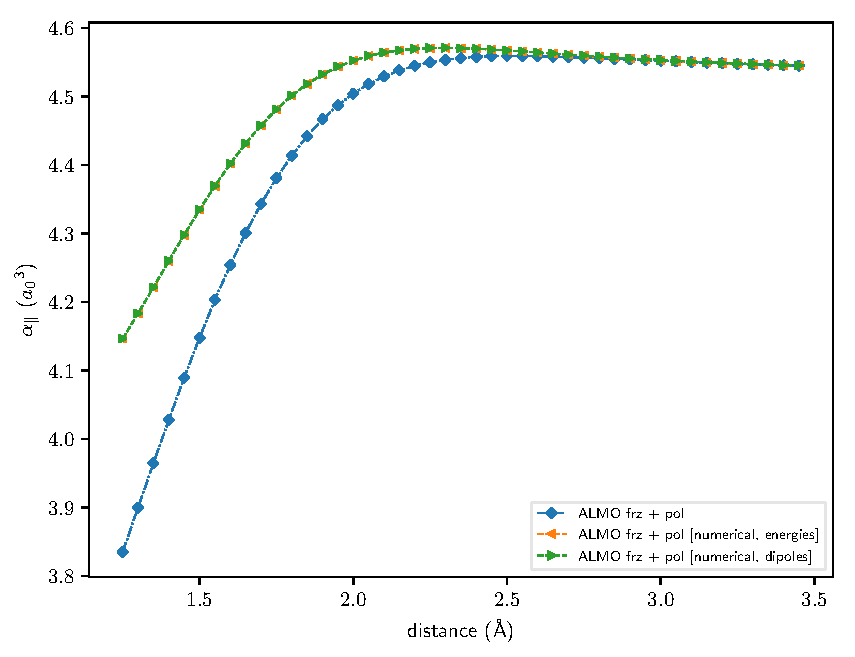
\includegraphics[scale=0.90]{almo_analytic_vs_numerical_onaxis_projected_short_def2-SVP.pdf}
  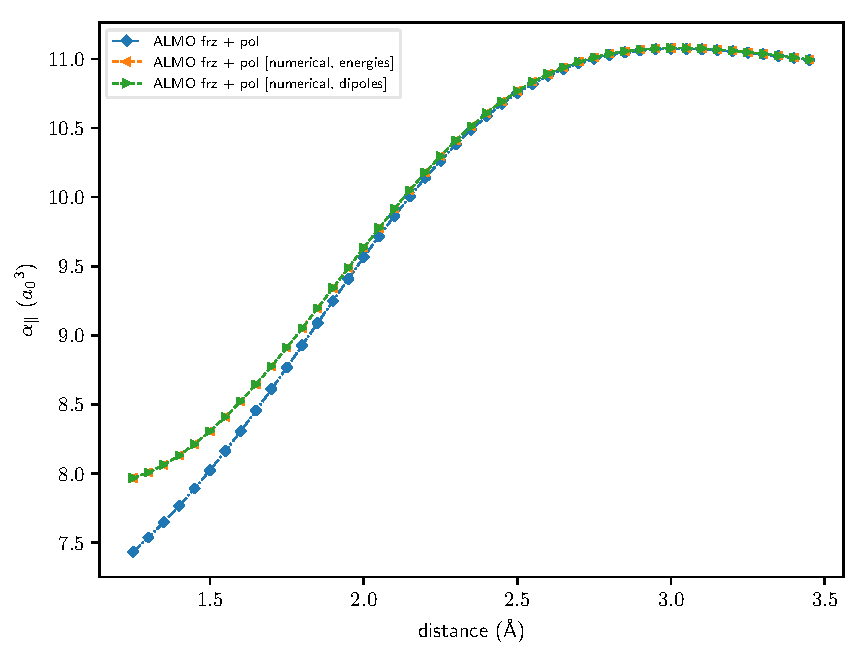
\includegraphics[scale=0.90]{almo_analytic_vs_numerical_onaxis_projected_short_def2-SVPD.pdf}
  \caption[Distance dependence of analytic and numerical ALMO polarizabilities]{Distance dependence of analytic and numerical ALMO polarizabilities for both basis sets.}
  \label{fig:distance-dependence-validation}
\end{figure}

\begin{figure}
  \centering
  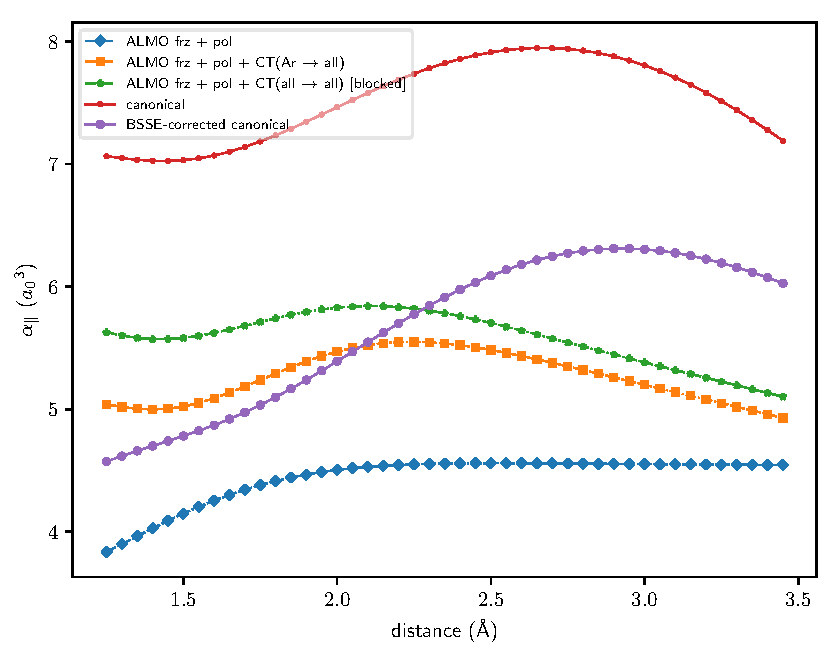
\includegraphics[scale=0.90]{almo_vs_bsse_canonical_onaxis_projected_short_def2-SVP.pdf}
  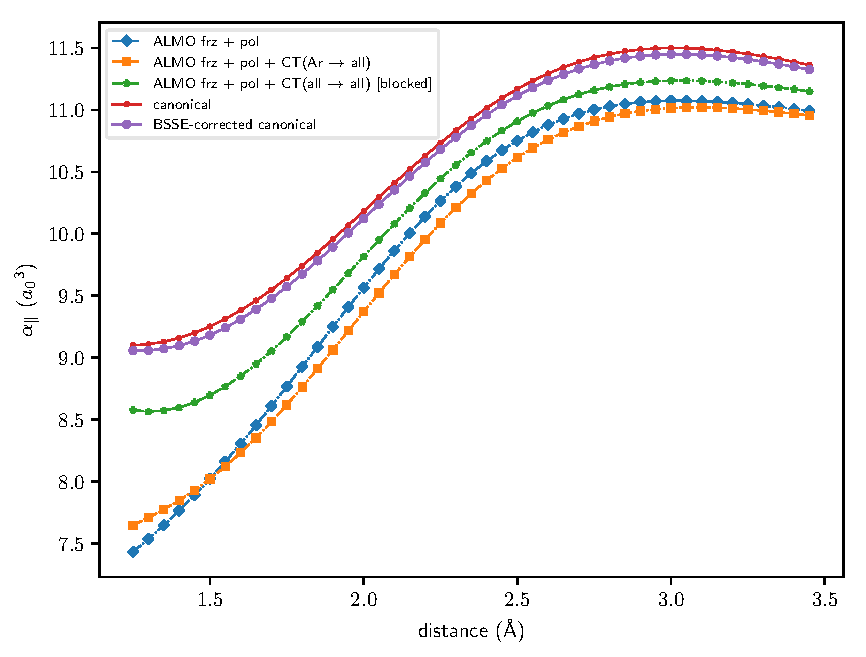
\includegraphics[scale=0.90]{almo_vs_bsse_canonical_onaxis_projected_short_def2-SVPD.pdf}
  \caption[Distance dependence of CT restrictions on polarizabilities]{Distance dependence of CT restrictions on polarizabilities for both basis sets.}
  \label{fig:distance-dependence-ct-levels}
\end{figure}

Figure~\ref{fig:distance-dependence-ct-levels} shows how the different forms of CT restriction vary as a function of interatomic distance. Similar to the counterpoise (CP) correction for interaction energies, the ``BSSE-corrected canonical'' polarizability for two monomers A and B is defined as
\begin{equation}
  \alpha^{\text{BSSE-corrected}} = \alpha^{AB}(AB) - \left[ \left( \alpha^{A}(AB) - \alpha^{A}(A) \right) + \left( \alpha^{B}(AB) - \alpha^{B}(B) \right) \right],
  \label{eq:bsse-corrected-polarizability}
\end{equation}
where, for example, \(\alpha^{A}(AB)\) is the polarizability of monomer A in the combined (supermolecular) basis of both monomers.

The difference from the BSSE correction is large in def2-SVP but negligible in def2-SVPD, confirming our results from section~\ref{sssec:basis-set-dependence}. For both basis sets, the argon polarizability is the major contributor, provided that the entire dimer basis virtual space is available. The difference between the argon and blocked ALMO curves is due to the small but non-zero polarizability of the lithium cation, plus a mutual or higher-order polarization effect that appears at shorter than equilibrium distances for def2-SVP. Most notably, there is a quantitative difference between the blocked ALMO and canonical results even with def2-SVPD, showing that the wavefunction mechanism is large, and only allowing CT during the response calculation cannot recover these effects.

\section{\texorpdfstring{\caps{Conclusions and Future Work}}{Conclusions and Future Work}}
\label{sec:conclusions-and-future-work}

We have presented an implementation of linear response molecular properties for ALMOs, along with a decomposition of charge transfer effects, applied to a system with a substantial CT interaction. We discovered that for the static polarizability, charge transfer plays an equally important role in the response calculation as it does in the underlying wavefunction. Additionally, our results confirm that the ALMO and LR(MI) approximations are valid as long as the basis set is not deficient for the system, as is the case with def2-SVP.

A question not addressed in this work or other ALMO-based work on excitation energies\cite{Closser_2015_5791,doi:10.1063/1.4926837} is the effect of non-locality on the projected virtual space. To properly assign fragment-localized contributions to molecular response, both the occupied and virtual ALMOs must be spatially localized to individual fragments. Projecting the occupied space out of the virtual space ensures occupied-virtual orthogonality between fragments, but removes the fragment locality of the virtual space; that is, each virtual MO can no longer be uniquely assigned to a specific fragment. However, we expect that the error introduced by a delocalized virtual space is small compared to the error from using unprojected orbitals, which are less representative of the true potential energy surface for the reasons discussed in section~\ref{ssec:almo-adaptation}. Future work will use LoProp-type approaches on top of projected ALMOs to investigate the magnitude of these effects. In this way, LR(MI) can be a sensitive test for how modification of the virtual space affects molecular properties.

Our development of a library for calculating molecular response properties of arbitrary operators with non-orthogonal orbitals opens many doors for future development. \libresponse{} is available in \qchem{} 5.0.2 and at \url{https://github.com/LambrechtLab/libresponse} under the 3-clause BSD license as an Armadillo-based\cite{armadillo} C++ library. It can also be used as a \psif{}\cite{Psi41.1} plugin.

\section{\texorpdfstring{\caps{Acknowledgements}}{Acknowledgements}}

E.J.B. thanks \qchem{} for a summer internship opportunity, Evgeny Epifanovsky for help with the initial DIIS implementation, and cclib\cite{OBoyle:2008cc,eric_berquist_2016_60670} for the analysis framework.

\section{\texorpdfstring{\caps{Supporting Information}}{Supporting Information}}

ALMO-EDA results and analysis, additional ghost basis and point charge analysis, additional distance dependence results, sample input files, pseudocode for algorithm.

\begin{table}
  \centering
  \caption[ALMO-EDA results for argon\textemdash{}lithium cation dimer]{ALMO-EDA results. Energy units are \si{\kcal\per\mol}. All calculations used Hartree-Fock with a bond length of \SI{2.4297}{\angstrom}.}
  \label{tab:almo-eda-results}
  \IfStandalone{\begin{tabular}{ccc}
\toprule
& \multicolumn{2}{c}{basis set} \\
ALMO-EDA term & def2-SVP & def2-SVPD \\
\midrule
\(\Delta E_{\textrm{frz}}\) & 1.20 & 2.18 \\
\(\Delta E_{\textrm{pol}}\) & -3.32 & -6.61 \\
\(\Delta E_{\textrm{del}}^{\textrm{RS}}\) & -4.07 & -0.89 \\
\(\Delta E_{\textrm{BSSE}}^{\textrm{RS}}\) & 1.38 & 0.16 \\
\(\Delta E_{\textrm{CT}}^{\textrm{RS}}\) & -2.69 & -0.74 \\
\(\Delta E_{\textrm{int}}^{\textrm{RS}}\) & -4.81 & -5.17 \\
\(\Delta E_{\textrm{del}}^{\textrm{SCF}}\) & -5.38 & -1.08 \\
\(\Delta E_{\textrm{BSSE}}^{\textrm{SCF}}\) & 1.79 & 0.16 \\
\(\Delta E_{\textrm{CT}}^{\textrm{SCF}}\) & -3.59 & -0.91 \\
\(\Delta E_{\textrm{int}}^{\textrm{SCF}}\) & -5.70 & -5.35 \\
\(\Delta E_{\textrm{HO}}^{\textrm{SCF}}\) & -0.90 & -0.18 \\
\bottomrule
\end{tabular}
}{\begin{tabular}{ccc}
\toprule
& \multicolumn{2}{c}{basis set} \\
ALMO-EDA term & def2-SVP & def2-SVPD \\
\midrule
\(\Delta E_{\textrm{frz}}\) & 1.20 & 2.18 \\
\(\Delta E_{\textrm{pol}}\) & -3.32 & -6.61 \\
\(\Delta E_{\textrm{del}}^{\textrm{RS}}\) & -4.07 & -0.89 \\
\(\Delta E_{\textrm{BSSE}}^{\textrm{RS}}\) & 1.38 & 0.16 \\
\(\Delta E_{\textrm{CT}}^{\textrm{RS}}\) & -2.69 & -0.74 \\
\(\Delta E_{\textrm{int}}^{\textrm{RS}}\) & -4.81 & -5.17 \\
\(\Delta E_{\textrm{del}}^{\textrm{SCF}}\) & -5.38 & -1.08 \\
\(\Delta E_{\textrm{BSSE}}^{\textrm{SCF}}\) & 1.79 & 0.16 \\
\(\Delta E_{\textrm{CT}}^{\textrm{SCF}}\) & -3.59 & -0.91 \\
\(\Delta E_{\textrm{int}}^{\textrm{SCF}}\) & -5.70 & -5.35 \\
\(\Delta E_{\textrm{HO}}^{\textrm{SCF}}\) & -0.90 & -0.18 \\
\bottomrule
\end{tabular}
}
\end{table}

\begin{table}
  \centering
  \caption{Analysis of ALMO-EDA terms from table~\ref{tab:almo-eda-results}.}.
  \label{tab:almo-eda-results-percentages}
  \IfStandalone{\begin{tabular}{ccc}
\toprule
& \multicolumn{2}{c}{basis set} \\
& def2-SVP & def2-SVPD \\
\midrule
\(\Delta E_{\textrm{pol}}\) + \(\Delta E_{\textrm{CT}}^{\textrm{RS}}\) (kcal/mol) & -6.01 & -7.34 \\
\(\Delta E_{\textrm{pol}}\) + \(\Delta E_{\textrm{CT}}^{\textrm{SCF}}\) (kcal/mol) & -6.91 & -7.52 \\
100 * \(\Delta E_{\textrm{BSSE}}^{\textrm{RS}}\) / \(\Delta E_{\textrm{CT}}^{\textrm{RS}}\) (\%) & -51.4 & -21.2 \\
100 * \(\Delta E_{\textrm{BSSE}}^{\textrm{SCF}}\) / \(\Delta E_{\textrm{CT}}^{\textrm{SCF}}\) (\%) & -49.9 & -17.7 \\
100 * \(\Delta E_{\textrm{CT}}^{\textrm{RS}}\) / (\(\Delta E_{\textrm{pol}}\) + \(\Delta E_{\textrm{CT}}^{\textrm{RS}}\)) (\%) & 44.8 & 10.0 \\
100 * \(\Delta E_{\textrm{CT}}^{\textrm{SCF}}\) / (\(\Delta E_{\textrm{pol}}\) + \(\Delta E_{\textrm{CT}}^{\textrm{SCF}}\)) (\%) & 51.9 & 12.2 \\
\bottomrule
\end{tabular}
}{\begin{tabular}{ccc}
\toprule
& \multicolumn{2}{c}{basis set} \\
& def2-SVP & def2-SVPD \\
\midrule
\(\Delta E_{\textrm{pol}}\) + \(\Delta E_{\textrm{CT}}^{\textrm{RS}}\) (kcal/mol) & -6.01 & -7.34 \\
\(\Delta E_{\textrm{pol}}\) + \(\Delta E_{\textrm{CT}}^{\textrm{SCF}}\) (kcal/mol) & -6.91 & -7.52 \\
100 * \(\Delta E_{\textrm{BSSE}}^{\textrm{RS}}\) / \(\Delta E_{\textrm{CT}}^{\textrm{RS}}\) (\%) & -51.4 & -21.2 \\
100 * \(\Delta E_{\textrm{BSSE}}^{\textrm{SCF}}\) / \(\Delta E_{\textrm{CT}}^{\textrm{SCF}}\) (\%) & -49.9 & -17.7 \\
100 * \(\Delta E_{\textrm{CT}}^{\textrm{RS}}\) / (\(\Delta E_{\textrm{pol}}\) + \(\Delta E_{\textrm{CT}}^{\textrm{RS}}\)) (\%) & 44.8 & 10.0 \\
100 * \(\Delta E_{\textrm{CT}}^{\textrm{SCF}}\) / (\(\Delta E_{\textrm{pol}}\) + \(\Delta E_{\textrm{CT}}^{\textrm{SCF}}\)) (\%) & 51.9 & 12.2 \\
\bottomrule
\end{tabular}
}
\end{table}

\begin{table}
  \centering
  \caption[Point charge and ghost function polarizability analysis]{Percentage of supermolecular result for point charge and ghost function polarizabilities. All calculations used Hartree-Fock with canonical MOs and a distance of \SI{2.4297}{\angstrom} from argon to the other center(s).}
  \label{tab:basis-set-dependence-percentages}
  \IfStandalone{\begin{tabular}{llrrrrr}
\toprule
 basis set &                          structure & \(\alpha_{\perp}\) & \(\alpha_{\parallel}\) & \(\bar{\alpha}\) & \(^{\text{t}}E_{0 \rightarrow \text{lowest}}^{\text{RPA}}\) & \(^{\text{s}}E_{0 \rightarrow \text{lowest}}^{\text{RPA}}\) \\
\midrule
  def2-SVP &   \ce{Ar\bond{....}PC(\mathrm{-})} &               84.1 &                   55.2 &             71.6 &                                                       195.5 &                                                       206.0 \\
  def2-SVP &                            \ce{Ar} &               83.9 &                   55.5 &             71.6 &                                                       199.1 &                                                       209.4 \\
  def2-SVP &   \ce{Ar\bond{....}PC(\mathrm{+})} &               83.7 &                   55.6 &             71.6 &                                                       196.8 &                                                       207.2 \\
  def2-SVP &  \ce{Ar\bond{....}\mathrm{Gh}(Li)} &               93.9 &                   79.1 &             87.5 &                                                       103.0 &                                                       103.3 \\
 def2-SVPD &   \ce{Ar\bond{....}PC(\mathrm{-})} &              108.6 &                   93.4 &            103.3 &                                                        91.2 &                                                        94.7 \\
 def2-SVPD &                            \ce{Ar} &              103.0 &                   93.8 &             99.7 &                                                       105.3 &                                                       107.1 \\
 def2-SVPD &   \ce{Ar\bond{....}PC(\mathrm{+})} &               99.7 &                  108.0 &            102.6 &                                                        82.6 &                                                        84.9 \\
 def2-SVPD &  \ce{Ar\bond{....}\mathrm{Gh}(Li)} &              103.2 &                   94.2 &            100.0 &                                                       100.6 &                                                       100.6 \\
\bottomrule
\end{tabular}
}{\begin{tabular}{llrrrrr}
\toprule
 basis set &                          structure & \(\alpha_{\perp}\) & \(\alpha_{\parallel}\) & \(\bar{\alpha}\) & \(^{\text{t}}E_{0 \rightarrow \text{lowest}}^{\text{RPA}}\) & \(^{\text{s}}E_{0 \rightarrow \text{lowest}}^{\text{RPA}}\) \\
\midrule
  def2-SVP &   \ce{Ar\bond{....}PC(\mathrm{-})} &               84.1 &                   55.2 &             71.6 &                                                       195.5 &                                                       206.0 \\
  def2-SVP &                            \ce{Ar} &               83.9 &                   55.5 &             71.6 &                                                       199.1 &                                                       209.4 \\
  def2-SVP &   \ce{Ar\bond{....}PC(\mathrm{+})} &               83.7 &                   55.6 &             71.6 &                                                       196.8 &                                                       207.2 \\
  def2-SVP &  \ce{Ar\bond{....}\mathrm{Gh}(Li)} &               93.9 &                   79.1 &             87.5 &                                                       103.0 &                                                       103.3 \\
 def2-SVPD &   \ce{Ar\bond{....}PC(\mathrm{-})} &              108.6 &                   93.4 &            103.3 &                                                        91.2 &                                                        94.7 \\
 def2-SVPD &                            \ce{Ar} &              103.0 &                   93.8 &             99.7 &                                                       105.3 &                                                       107.1 \\
 def2-SVPD &   \ce{Ar\bond{....}PC(\mathrm{+})} &               99.7 &                  108.0 &            102.6 &                                                        82.6 &                                                        84.9 \\
 def2-SVPD &  \ce{Ar\bond{....}\mathrm{Gh}(Li)} &              103.2 &                   94.2 &            100.0 &                                                       100.6 &                                                       100.6 \\
\bottomrule
\end{tabular}
}
\end{table}

\begin{figure}
  \centering
  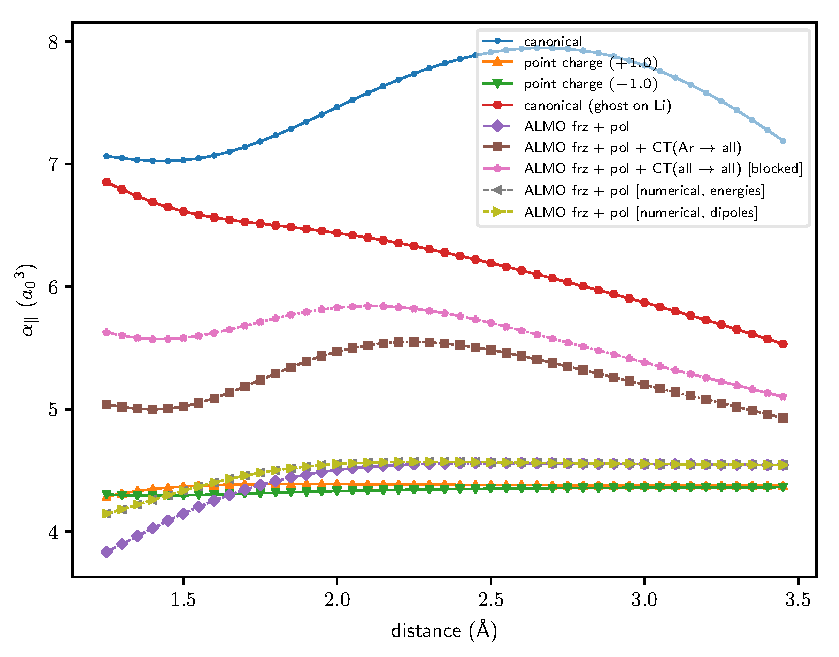
\includegraphics[scale=0.90]{polar_onaxis_projected_short_def2-SVP.pdf}
  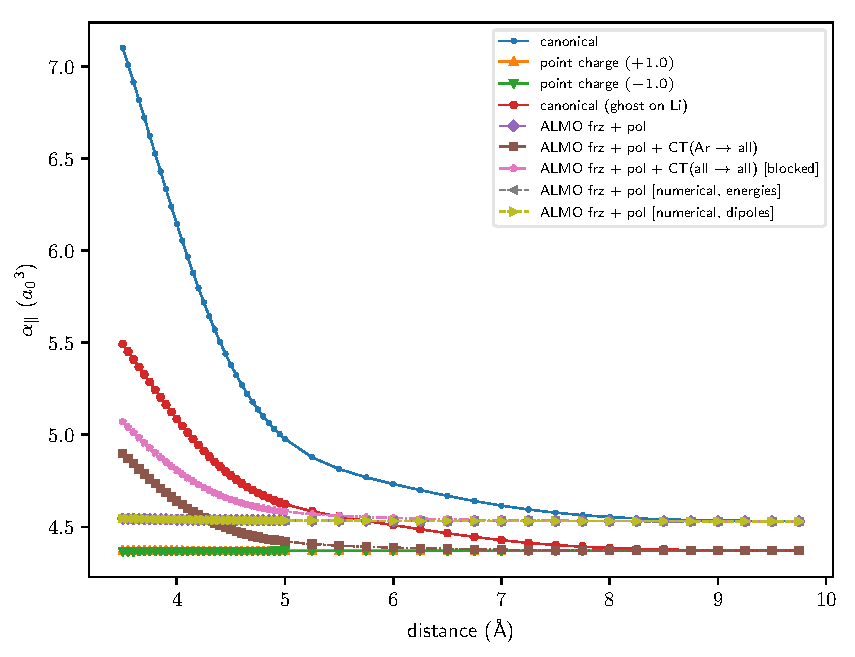
\includegraphics[scale=0.90]{polar_onaxis_projected_long_def2-SVP.pdf}
  \caption[Distance dependence of \(\alpha_{\parallel}\) for def2-SVP]{Short- and long-range interatomic separation dependence of the static polarizability parallel to the coordination axis. All calculations are at the HF/def2-SVP level.}
  \label{fig:distance-dependence-parallel-def2-svp}
\end{figure}

\begin{figure}
  \centering
  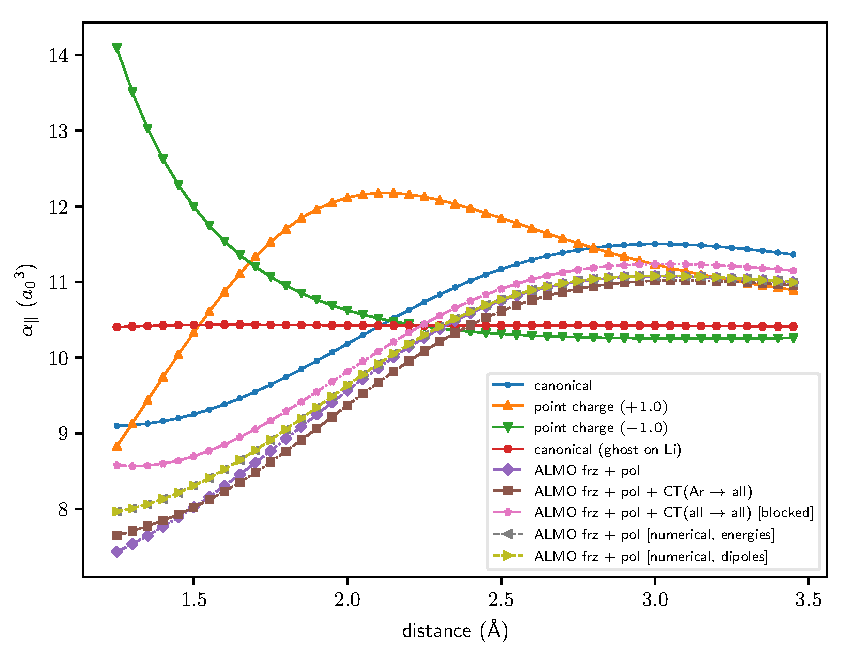
\includegraphics[scale=0.90]{polar_onaxis_projected_short_def2-SVPD.pdf}
  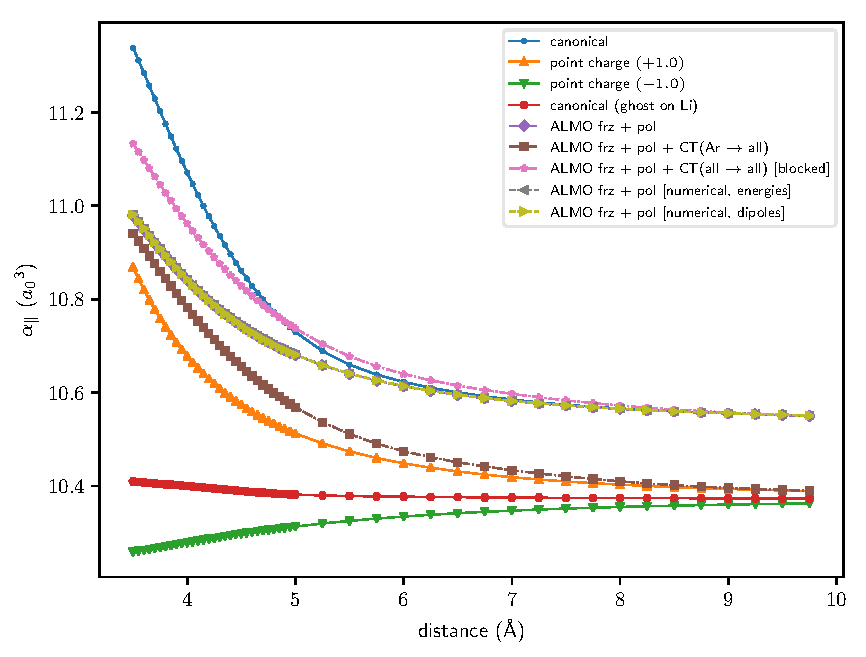
\includegraphics[scale=0.90]{polar_onaxis_projected_long_def2-SVPD.pdf}
  \caption[Distance dependence of \(\alpha_{\parallel}\) for def2-SVPD]{Short- and long-range interatomic separation dependence of the static polarizability parallel to the coordination axis. All calculations are at the HF/def2-SVPD level.}
  \label{fig:distance-dependence-parallel-def2-svpd}
\end{figure}

\begin{figure}
  \centering
  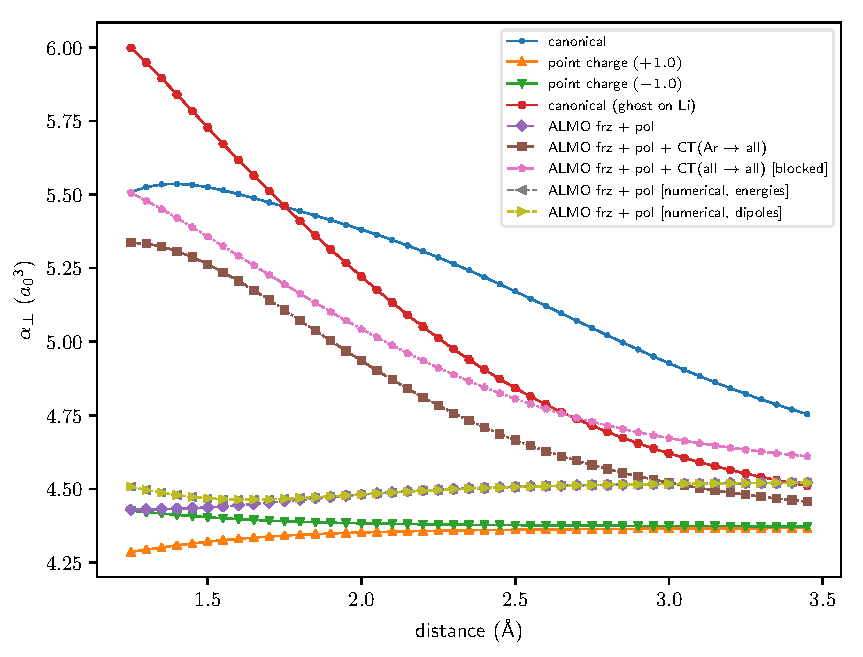
\includegraphics[scale=0.90]{polar_offaxis_projected_short_def2-SVP.pdf}
  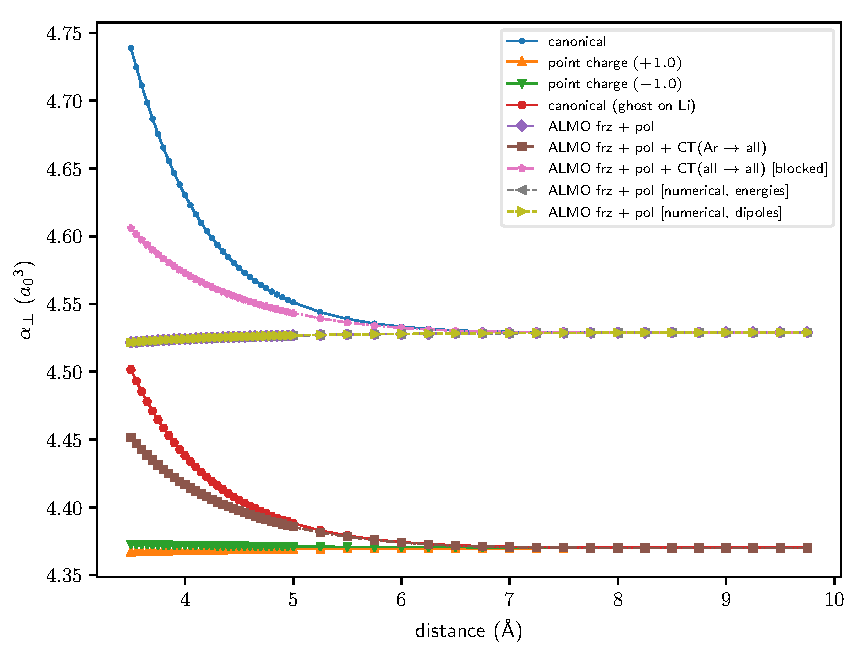
\includegraphics[scale=0.90]{polar_offaxis_projected_long_def2-SVP.pdf}
  \caption[Distance dependence of \(\alpha_{\perp}\) for def2-SVP]{Short- and long-range interatomic separation dependence of the static polarizability perpendicular to the coordination axis. All calculations are at the HF/def2-SVP level.}
  \label{fig:distance-dependence-perp-def2-svp}
\end{figure}

\begin{figure}
  \centering
  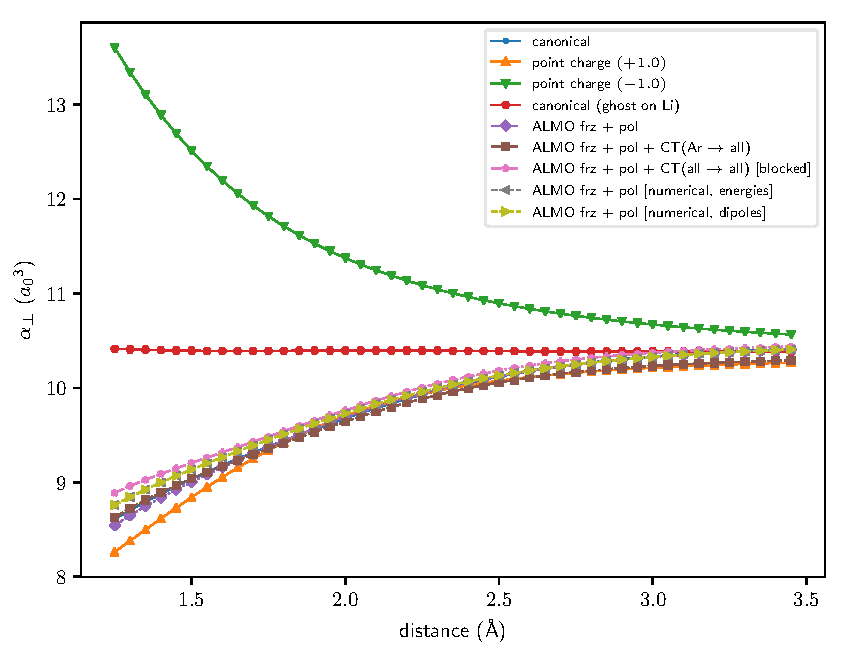
\includegraphics[scale=0.90]{polar_offaxis_projected_short_def2-SVPD.pdf}
  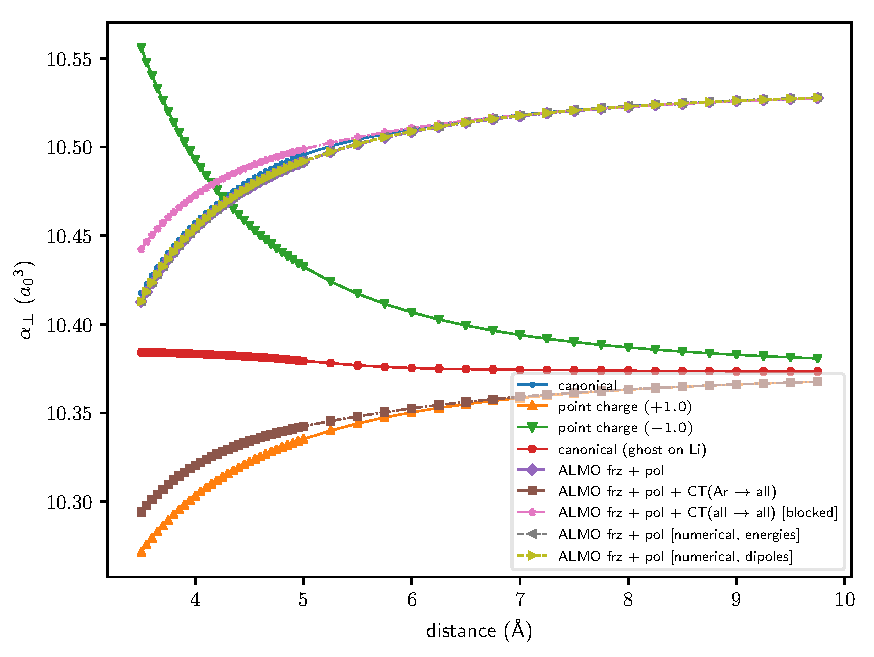
\includegraphics[scale=0.90]{polar_offaxis_projected_long_def2-SVPD.pdf}
  \caption[Distance dependence of \(\alpha_{\perp}\) for def2-SVPD]{Short- and long-range interatomic separation dependence of the static polarizability perpendicular to the coordination axis. All calculations are at the HF/def2-SVPD level.}
  \label{fig:distance-dependence-perp-def2-svpd}
\end{figure}

As a sanity check for all results, we expect certain physical behavior over the range of interatomic distances. In particular, as the interatomic distance approaches the limit of infinite separation,

\begin{itemize}
\item The canonical SCF, numerical SCF(MI), and analytic SCF(MI) results all converge to the same value, which is the sum of polarizabilities the two isolated atoms. CT appears to be an important contributor until approximately \SI{5}{\angstrom}, where the decay behavior of the canonical SCF changes.
\item The point charge, and ``frz + pol + CT(\ce{Ar} \(\rightarrow\) all)'' results all converge to the same value, which is the polarizability of the isolated argon atom.
\end{itemize}

\subsection{Input files}

\lstinputlisting[%
frame=single,%
label=listing:input-polarizability,%
caption=Sample \qchem{} input file for ``ALMO frz + pol'' polarizability. Geometry is from HF/def2-SVPD.%
]{\IfStandalone{almo_stoll_projvirts_restricted.in}{paper_04/almo_stoll_projvirts_restricted.in}}

Using the template from listing~\ref{listing:input-polarizability}:

\begin{itemize}
\item To perform the ``ALMO frz + pol + CT(all \(\rightarrow\) all) [blocked]'' calculations, set \\
  \lstinline|_frgm_response_idx = 0| and all \lstinline|_mask_*| options to \lstinline|false|.
\item To perform the ``ALMO frz + pol + CT(Ar \(\rightarrow\) all)'' calculations, set \\
  \lstinline|_frgm_response_idx = 1| and all \lstinline|_mask_*| options to \lstinline|true|.
\end{itemize}

\lstinputlisting[%
frame=single,%
label=listing:input-almo-eda-gen1,%
caption=Sample \qchem{} input file for first-generation ALMO-EDA. Geometry is from HF/def2-SVPD.%
]{\IfStandalone{eda_bsse_def2-SVPD.in}{paper_04/eda_bsse_def2-SVPD.in}}

\lstinputlisting[%
frame=single,%
label=listing:input-almo-eda-gen2,%
caption=Sample \qchem{} input file for second-generation ALMO-EDA. Geometry is from HF/def2-SVP.%
]{\IfStandalone{eda2_1_scf_nobsse_def2-SVPD.in}{paper_04/eda2_1_scf_nobsse_def2-SVPD.in}}

\subsection{Algorithm description}

\algnewcommand\Break{\textbf{break}}
\algnewcommand\Not{\textbf{not}}
\algnewcommand\True{\textbf{true}}
\algnewcommand\False{\textbf{false}}
\algnewcommand\Rhsvecs{\textsf{rhsvecs}}
\algnewcommand\Rspvecs{\textsf{rspvecs}}
\algnewcommand\Operators{\textsf{operators}}
\algnewcommand\Resp{\textsf{resp}}
\algnewcommand\AllowCT{\textsf{allow\_ct?}}

\begin{algorithm}
  \centering
  \begin{algorithmic}[1]
  \Procedure{solve\_linear\_response}{\Resp, \Operators, occupations, \(\mat{C}, \mat{F}, \mat{S}, \vartheta\), maxiter, \AllowCT}
  \For{\(s \gets 1, N_{spin}\)}
    \State Transformation of \(\mat{F}\) and \(\mat{S}\) from AO to full MO basis
    \State \(E_{ia,jb} = F_{ab}S_{ij} - F_{ij}S_{ab}\)
    \Comment{Form non-orthogonal orbital energy matrix \(\mat{E}\)}
    \If{\Not{} \AllowCT{}}
      \State Zero cross-fragment \(ia\) indices and shrink dimensions of \(\mat{E}\)
    \EndIf
    \State Form inverse for denominator \(\mat{E}^{-1}\)
  \EndFor
  \For{\(i \gets 1, N_{operators}\)}
    \For{\(c \gets 1, N_{components}\)}
      \State \((\mat{Z})_{\mu\nu} \gets \Operators[i,c,\mu\nu]\)
      \Comment{Select operator component as perturbation for right-hand side}
      \State Transform operator component from AO to occ-virt MO basis and append \(\mat{Z}_{ia}\) to \Rhsvecs
      \If{\Not{} \AllowCT{}}
        \State Zero cross-fragment \(ia\) indices and shrink dimensions of \(\mat{Z}\)
      \EndIf
      \State \(\mat{X}^{(0)} \gets \mat{0}\)
      \Comment{Form initial guess for response vector (uncoupled result)}
      \State \(converged \gets \False\)
      \For{\(n \gets 1, maxiter\)}
        \State \(D_{\mu\nu}^{X} \gets C_{\mu i} X_{ia}^{(n-1)} C_{\nu a}\)
        \Comment{Form perturbed density}
        \State \(J_{\mu\nu}^{X}\left[\mat{D}^{X}\right], K_{\mu\nu}^{X}\left[\mat{D}^{X}\right] \gets fock\_build(\mat{D}^{X})\)
        \Comment{Form Coulomb and exchange contributions}
        \State \(\left(\mat{R}^{(n)}\right)_{\mu\nu} \gets 4 \mat{J}^{X} - \mat{K}^{X} - \left(\mat{K}^{X}\right)^{T}\)
        \Comment{Form half-transformed orbital Hessian-vector product (here, \(\mat{G} = \mat{A}^{s} + \mat{B}^{s}\))}
        \State Do second transformation of Hessian-vector product \(\left(\mat{R}\right)_{ia}^{(n)}\)
        \If{\Not{} \AllowCT{}}
          \State Zero cross-fragment \(ia\) indices and shrink dimensions of \(\mat{R}, \mat{X}\)
        \EndIf
        \State \(X_{ia}^{(n)} \gets (\mat{E}^{-1})_{ia,jb} \left[ Z_{jb} - R_{jb}^{(n)} \right]\)
        \Comment{Update response vector}
        \If{\Not{} \AllowCT{}}
          \State Restore dimensions of \(\mat{X}\)
        \EndIf
        \If{\(||\mat{X}^{(n)} - \mat{X}^{(n-1)}|| < \vartheta\)}
          \State \(converged \gets \True\)
          \State Append \(\mat{X}^{(n)}\) to \Rspvecs
          \State \Break
        \EndIf
  \algstore{lrmi}
  \end{algorithmic}
  \caption{Static linear response approach within fragment-localized formalism.}
  \label{alg:solve-linear-response}
\end{algorithm}
\begin{algorithm}
  \centering
  \begin{algorithmic}[1]
  \algrestore{lrmi}
        \EndFor
      \If{\Not{} \(converged\)}
        \State crash
      \EndIf
    \EndFor
  \EndFor
  \State \(\Resp \gets \mat{0}\)
  \Comment{Form all possible permutations of property gradient and response vectors}
  \For{\(a \gets 1, len(\Rhsvecs)\)}
    \For{\(b \gets 1, len(\Rspvecs)\)}
      \State \(\mat{P} \gets \Rhsvecs[a], \mat{Q} \gets \Rspvecs[b]\)
      \State \(\lr{P}{Q}_{0} \gets -P_{ia}Q_{ia}\)
      \State \(\Resp[a,b] \gets \lr{P}{Q}_{0}\)
    \EndFor
  \EndFor
  \EndProcedure
  \end{algorithmic}
  \caption{Continuation of algorithm~\ref{alg:solve-linear-response}}
  \label{alg:solve-linear-response-2}
\end{algorithm}

Algorithm~\ref{alg:solve-linear-response}/\ref{alg:solve-linear-response-2} is the general outline of the LR(MI) procedure, without convergence acceleration. The key difference between our implementation and a general CPHF solver is the zeroing of vector and matrix elements. Again, any contraction between \(ia\) or \(ia,jb\) indices may be restricted, but transformations from \(\mu\nu\) to \(ia\) are not.

Missing from this example is the formation of \(\mat{A}, \mat{B}\), and the prefactor in the equation for real/imaginary operators. A difference from the paper equations in the implementation is that rather than take a single \(\op{P}\) and single \(\op{Q}\), a list of operators is passed. For example, if \(\Operators = [\op{\mu}, \op{m}]\), then \(\lr{\mu}{\mu},\lr{\mu}{m}\), and \(\lr{m}{m}\) will automatically be formed. Another implementation detail is that each operator carries its own property gradient vectors (the occ-virt MO basis integrals for the right-hand side) and perturbed response vectors, and each operator carries information about whether it is real/imaginary and spin conserving/altering.
\onlyifstandalone{\printbibliography}
\end{document}
